\chapter{Introduction and Preliminary Research}\label{introduction,research}\label{section \thechapter}

\mySection{Project brief}{writer TBA}\label{project brief}
    \towrite{project brief}

\mySection{Art review}{\AH, \AR}\label{art review}
    \begin{figure}%{I}{0.45\textwidth}
        % \vspace{-11pt}
        \centering
        \begin{subfigure}[b]{0.45\textwidth}
            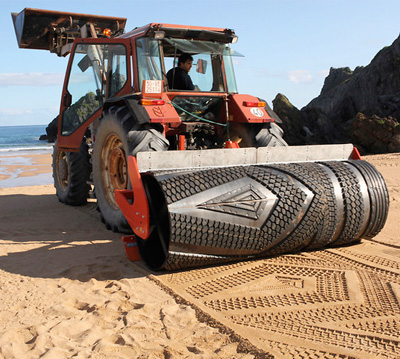
\includegraphics[width=\textwidth]{Files/sand_machine.jpg}
            \caption{Sand-printing tractor. The roller on the front produces the imprints.}
            \label{fig: sand machine}
        \end{subfigure}
        ~
        \begin{subfigure}[b]{0.45\textwidth}
            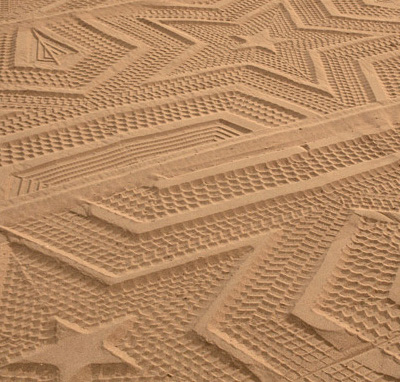
\includegraphics[width=\textwidth]{Files/sand_machine_art.jpg}
            \caption{Large-scale imprints produced using the tractor.}
            \label{fig: sand machine art}
        \end{subfigure}
        \caption{Gunilla Klingberg's `sand machine' and the pattern it produces. \small (Retrieved from     \citen{ShiMin2013} on 2016--01--20)}
        \label{fig: sand machine and art}
        % \vspace{-20pt}
    \end{figure}
    Land art (or Earth art) utilizes the landscape itself to produce the art. Structures are often made by placing natural materials, such as rocks or twigs, onto the land to form a pattern or picture. Another way they are produced is by sculpting the land to form patterns. The art is not simply placed onto the land, rather the land is the means of the creation. Pieces are often ephemeral in nature, being left to erode due to natural conditions over time, and so now only exist in photographic and video documentation.\\
    A significant inspiration for the creation of land art came from people's awareness of the negative impact they can have on the environment around them. By incorporating art into the natural landscape, artists hope that it will change people’s perspective of the environment around them.

    Land art is a largely American movement which began in the late 1960s. The movement is an offshoot of conceptualism and minimalism and was a protest to the commercialization of American art, leading the artists to produce works which were removed from the art market.\\
    It can be argued that land art was created by ancient cultures. Examples of land art occur around the world, such as the Nazca lines produced by the Nazca in southern Peru and The Great Serpent Mound in Ohio, US. It is believed that these pieces could have been created as a form of worship to the gods of the cultures which made these pieces.\\
    The modern movement began with the group exhibition ``Earth works'' in New York City in October 1968. In the following year, Willoughby Sharp curated the ``Earth Art'' exhibition at Cornell University which included many artists, such as Robert Smithson and Richard Long, who were big influences within the movement. Due to their monumental size the pieces were usually documented in photographs and maps which the artist could exhibit in a gallery. Land art was occasionally also produced within galleries; this was done by bringing in materials from the landscape and using them to create installations.\\
    %One of the most well-known artists in this movement was Robert Smithson. His best known piece, and possibly the most famous example of land art, is “Spiral Jetty” which was constructed in April 1970. It was constructed at Rozel Point, Great Salt Lake, Utah, reportedly this location was chosen by Smithson due to the blood red colour of the water which submerges the art at times of normal precipitation (the jetty is revealed during times of drought). The spiral structure was constructed using 6650 tons of black basalt rocks which were transported and manipulated in the lake bed using dumper trucks, tractors and front end loaders. The construction was documented and presented as a film, also called Spiral Jetty [3].


    \subsection{Sand art}\label{sand art}
        \begin{wrapfigure}{I}{0.45\textwidth}
            % \vspace{-11pt}
            \centering
            \begin{subfigure}[b]{0.45\textwidth}
                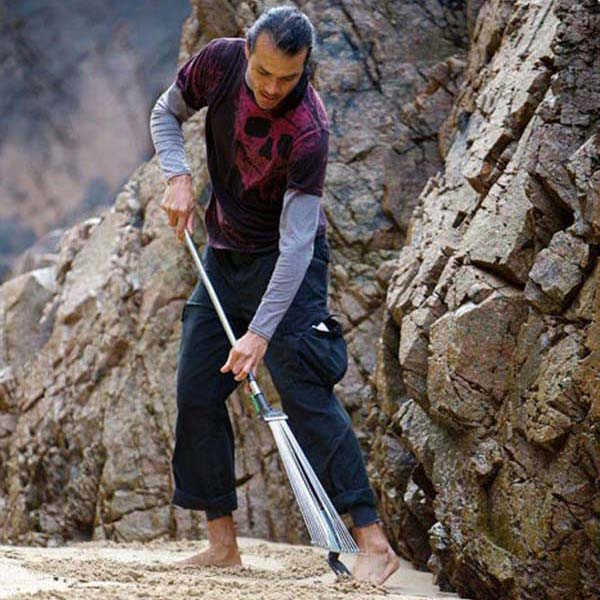
\includegraphics[width=\textwidth]{Files/andres_amador.jpg}
                \caption{Andres Amador using a rake to produce his playa pictures.}
                \label{fig: andres amador}
            \end{subfigure}
            \begin{subfigure}[b]{0.45\textwidth}
                
\includegraphics[width=\textwidth]{Files/andres_amador_art.jpg}
                \caption{Large-scale imprints produced using the tractor.}
                \label{fig: andres amador art}
            \end{subfigure}
            \caption{\small (Retrieved from \citen{andresamador} on 2016--01--23)}
            \label{fig: andres amador and art}
            % \vspace{-20pt}
        \end{wrapfigure}
        There are various styles of sand art; the main two are large scale sculptures and 2-dimensional freehand drawings. Over recent years smaller scale sand storytelling has developed which is concerned with both the performance and the final images produced. Large-scale artists mostly use easily accessible equipment such as shovels, buckets and rakes for freehand drawing and trowels and spatulas for sculpting. However, Swedish artist Gunilla Klingberg has developed a sand-printing tractor(Figure~\ref{fig: sand machine}), which produces large imprints across beaches (Figure~\ref{fig: sand machine art}). A low tide is needed for both printing and free hand drawing due to the wet sand.\\
        Jim Denevan, a popular freehand sand artist, ranges the scale of his work from small beach compositions to land works the size of a city. He has done live performances for exhibitions at Yerba Buena Centre for the Arts, 2005, and the Vancouver Sculpture Biennale, 2010. His work has also been featured in popular magazines such as the New York Times Magazine and National Geographic. Denevan does not use any sort of measuring tools and spends an average of 7 hours, walking about 30 miles, when producing his work. After all of this time his work is soon washed away by the incoming tide.\\
        Though the transient nature of this art form seems defeatist, it is actually the motivation for many sand artists. Andres Amador says he prefers a temporary medium and is much more concerned with his ``process and less about the result.'' He does not produce any form of permanent art work. Mr Amador's pieces, known as playa paintings, are produced using simply a rake and a rope as a guide (Figure~\ref{fig: andres amador and art}).

        Charlene Lanzel produces small-scale sand stories. Their creation can be observed as she creates images on a table top, projected onto a large screen sitting above her. Lanzel produces her images in darkness, the sand sitting on a glass table with lights underneath. Unlike other forms of sand art, her work is not washed away by the tide; instead she destroys the work herself in order to produce fluid images that play like an animation. Lanzel uses soundtracks alongside her performance to tell her stories and fully immerse her audience.

        Sand sculpture may be the largest scale form of sand art. Competitions are popular on beaches around the world and sculptures with the stature and solidity of woodcarvings are often produced.  Sculpture is also the most permanent style: many sculptures produced indoors last for more than a year.

\mySection{History of robotics}{\SW, \AK}\label{history of robotics}
    Autonomous robots have become common in many fields: factories make use of autonomous workers; space exploration vehicles include autonomous navigation systems and automated scientific instruments; military and commercial aircraft use autonomous systems to stay airborne; and large utilities providers (\eg water treatment plants and power stations) have some automated control systems.\\
    These technologies have been developing since the early 20th century. Some of those developments are of particular interest with regard to the development of a sand art--drawing robot.

    One difficult challenge in autonomous robotics is that of navigation. Many of the most advanced navigating robots that have been designed have been entrants in a Micromouse competition.\\
    The model of the Micromouse competition was introduced in 1977 by IEEE Spectrum magazine.\cite{harrison2010} It involves robots competing to get to the centre of a maze in the fastest time. There have been many variations of the rules, but the main theme is that the robots are autonomous. The inaugural competition was held in 1979 and was won by a high-speed dumb wall follower. In 1980 an entrant became the first Micromouse robot to find the centre of the maze and know it had done so, although it travelled at only \SI{0.2}{\meter\per\second}.

    Autonomous movement presents several other challenges. Many robots have been developed to move over different terrains. In particular these have been used to explore the surface of alien planets.\\
    The history of successful Mars rover missions began in 1997 with NASA's pathfinder mission. The `Pathfinder' lander contained a rover, `Sojourner', capable of exploring the martian surface. Sojourner succeeded in traveling 330 feet from the lander before it stopped communicating.\cite{MSUsojourner} Since then, NASA's Jet Propulsion Laboratory (JPL) has continued to develop robotic rovers for the unmanned exploration of Mars.\\
    Mars rovers must operate over sandy and rocky terrain. To facilitate this movement, all four rovers which have remained in communication with Earth for more than a day were equipped with 6 wheels. This locomotion mechanism was developed by testing the movement of rover prototypes in a Mars analog environment here on Earth. Given its similar terrain, the Mojave desert was selected. By the very nature of their missions, Mars rovers must operate far from human physical intervention and between 4 and 24 minutes behind instructions from Earth.\cite{Ormston}\\
    The motivation behind Mars rovers is two fold -- to complete scientific objectives to further improve our understanding of Mars and the solar system, and to complete mission objectives, improving the current state of space technology. Robotic rovers allow these objectives to be pursued (to varying degrees) without the risk of human life, and the far greater cost, of manned spaceflight.\\
    The latest rover to be sent to Mars, The Mars Science Laboratory (MSL), or `Curiosity', landed in August 2012.\cite{NASAcuriosity} It was deposited on the Martian surface by a vehicle called `Skycrane'. The Skycrane propulsively slowed Curiosity's decent, before lowering it to the ground by cables. Aboard Curiosity are instruments including cameras, radiation detectors and X-ray diffraction and spectrometry equipment. With this technology Curiosity is able to explore Mars and conduct scientific investigation.

    \mySubsection{Sand-drawing robots}{\SW}\label{sand-drawing robots}
        \begin{wrapfigure}{I}{0.45\textwidth}
          \begin{center}
            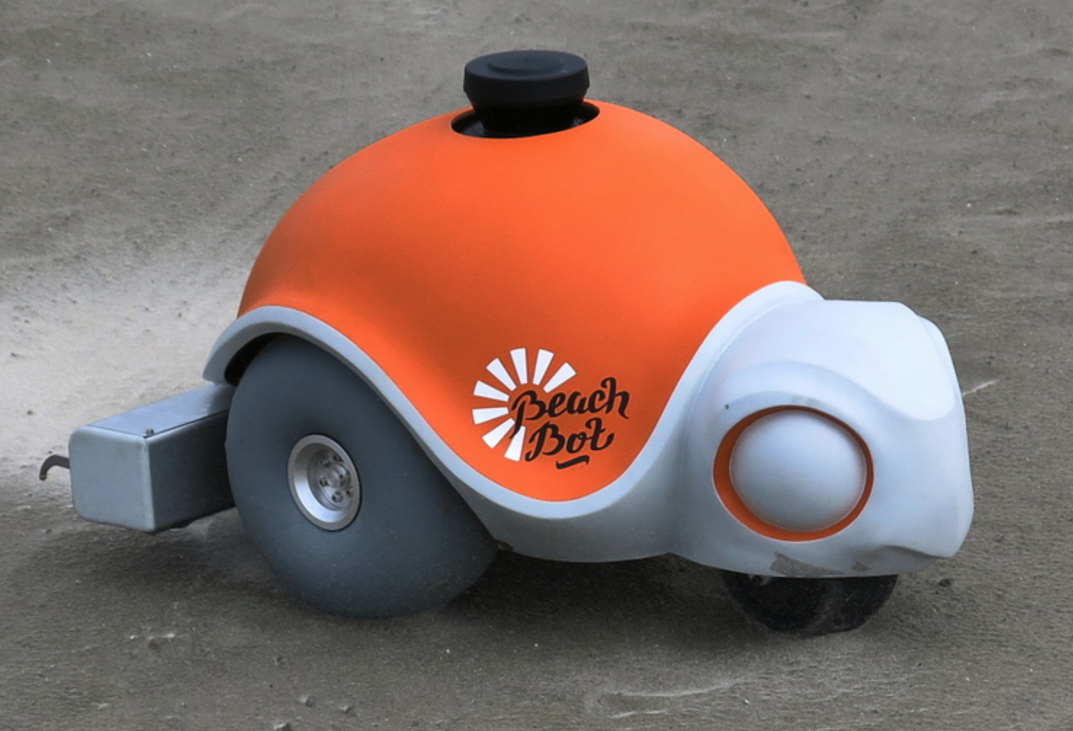
\includegraphics[width=0.43\textwidth]{Files/beachbot}
          \end{center}
          \caption{ETH Z\:urich's BeachBot robot.{\small (Retrieved from \citen{beachbot} on 2016--01--28)}}
          \label{fig: beachbot}
        \end{wrapfigure}
        The `best-in-class', and indeed only notable, beach-scale drawing robot is Disney's BeachBot (Figure~\ref{fig: beachbot}), produced by ETH Zurich.\cite{beachbot} The robot is capable of drawing images in the sand -- this has particular application in marketing Disney's sea themed--franchises and providing entertainment at Disney's beach resorts.\\
        The robot's drawing mechanism consists of fourteen rake teeth mounted in pairs on seven servo motors -- this allows lines of varying width (or no lines) to be drawn. The BeachBot is driven by two rear wheels and steered by a front wheel -- in a three-wheel configuration. It is fairly compact, measuring only sixty centimeters in length. BeachBot's chassis is enclosed in a sealed aluminum shell to protect its components from the sand. From this shell a laser scanner (part of BeachBot's guidance system) protrudes. The laser scanning guidance system directs BeachBot to draw its programmed image relative to reflecting posts installed by the user; this provides a `canvas' on which BeachBot works.\\
        BeachBot's shell is design to give it the appearance of a  turtle from Disney's \emph{Finding Nemo} property -- not only does this incorporate Disney's brand image into the design, but it also provides a non-threatening look. The latter point will be important for our robot since it will need to operate on a beach, an environment in which people are not used to seeing machinery.\\
        It has been suggested that with modification BeachBot could be used on snowy terrain to promote Disney's winter themed--franchises.

        \begin{wrapfigure}{O}{0.45\textwidth}
          \begin{center}
            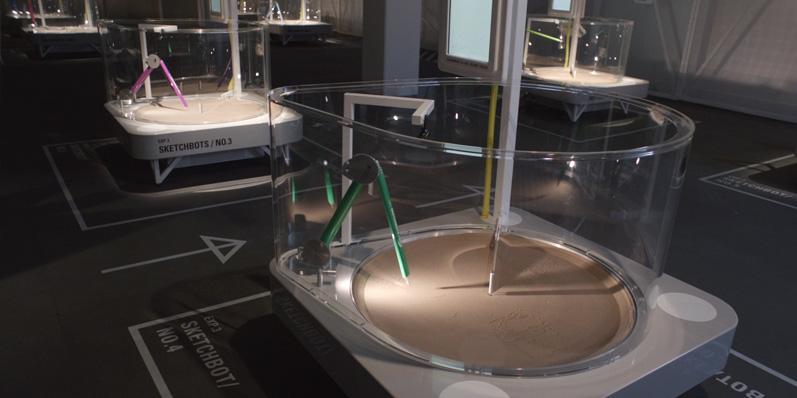
\includegraphics[width=0.43\textwidth]{Files/sketchbots}
          \end{center}
          \caption{Google Chrome Web Lab's sketchbots at the Science Museum, London.{\small (Retrieved from \citen{chromeweblab} on 2016--02--02)}}
          \label{fig: sketchbots}
        \end{wrapfigure}
        Although not beach-scale, Google has produced tabletop-scale sand art machines called `sketchbots' (Figure~\ref{fig: sketchbots}) (Operational at the Science Museum in London between 2012 and 2013).\cite{Warman2012} The robot itself was integrated with the tabletop; it comprised an arm with a mounted stylus and a `sweeping' implement, which moved in a circular motion, to clean the sand canvas. The robot took an input of the user's face from a camera, parsed the image and then drew it in the sand. Google  created the installation as part of its `Chrome Web Lab', showcasing modern web technologies such as HTML5.

\mySection{Robotics in education}{\SSB}\label{education review}
    The programming language Scratch was first released in 2005. It was designed by the Lifelong Kindergarten Group at the MIT Media Lab as a tool to introduce algorithmic thinking to 8--16 year-olds.\cite{scratch} The group state on their website that
    \begin{quotation}
        ``Scratch helps young people learn to think creatively, reason systematically, and work collaboratively -- essential skills for life in the 21st century.''
    \end{quotation}
    The inclusion of computational thinking in the primary science curriculum is gaining popularity. The ability to express the steps required to solve a given problem are important learning goals for children in a world where many rely on technology in the home, at work and in school.

    Furthermore, tools which allow students to employ these skills in the real world have proved to be very popular. The first programmable Lego product was released in 1989; since then the concept has been developed by numerous groups. Now there are several robotics platforms for educational purposes. The Lego group have several such platforms: the Lego Mindstorms range includes commercial packages as well as packages designed for schools. These allow high-school students to build embedded systems using different sensors and effectors to interact which can be programmed. The Mindstorms range forms the basis for the First Lego League competitions, which operate all over the world. MIT's Zero Robotics competitions also allow high- and middle-school students to program spherical robots on the International Space Station to solve challenges as part of an annual competition.\cite{zerorobotics}\\
    More recently, systems have been developed for younger students. Lego WeDo and WeDo 2.0 are designed for children aged 7--10 years to build simple robots and program them to perform actions using a software package based on Scratch.\cite{wedo2} This approach to robotics and programming has been designed in accordance with the US National Research Council's `Next Generation Science Standards'.

    \begin{wrapfigure}{I}{0.45\textwidth}
      \begin{center}
        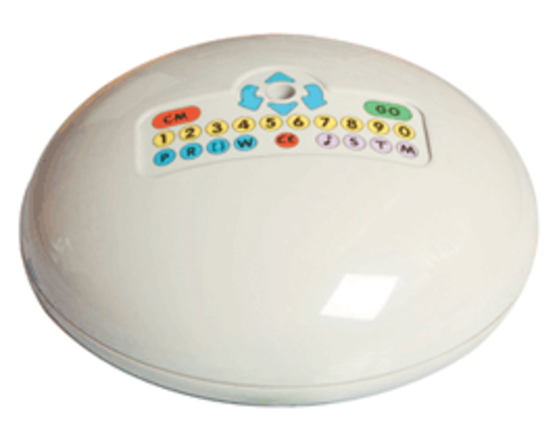
\includegraphics[width=0.43\textwidth]{Files/valiant_roamer.pdf}
      \end{center}
      \caption{The Valiant Technology Classic Roamer, a robot designed to teach algorithmic thinking to primary-age children. It is based on the Logo programming language. \small (Retrieved from \citen{valiantroamer} on 2015--01--18)}
      \label{fig: valiant roamer}
    \end{wrapfigure}
    However, none of the these technologies are new ideas: the programming language Logo was developed in 1967 as an educational tool. Among other features, Logo employed the idea of body-syntonic reasoning: processes are carried out relative to the current state, rather than relative to some reference state. One of Logo's creators, Seymour Papert, also invented a turtle robot (inspired by the tortoise robots developed by neurophysiologist William Grey Walter in the 1940s); this robot was programmed using Logo to move around a surface and draw patterns. It carried a pen and could be instructed to turn, move forwards and deploy or retract the pen. Using these simple commands, the turtle robot could be programmed to draw pictures and patterns on the surface over which it moved.\\
    Seymour Papert's turtles continue to be popular in primary schools across the world; the modern iteration is Valiant Technology's Roamer (Figure~\ref{fig: valiant roamer}).\cite{valiantroamer} Simple interfaces have been designed for the Roamer so it can be used without a programming language. Different models are available with different levels of complexity for different age ranges.
